\documentclass{article}
\usepackage[utf8]{inputenc}
\usepackage[russian]{babel}
\usepackage{amsfonts}
\usepackage{natbib}
\usepackage{upquote}
\usepackage{datetime}
\usepackage{multicol}
\usepackage{listings}
\usepackage{graphicx}

\setlength{\voffset}{-2cm}
\setlength{\textheight}{700pt}

\title{Численные методы: Лабораторная работа №3}
\author{Группа 4001BV: Карина Пилюшонока \and Александр Степанов \and Борис
Кувшинников} \date \today

\begin{document}
\maketitle
\newpage
\tableofcontents
\newpage
\section{Описание задачи}
Написать программную реализацию алгоритма для решения нелинейного уравнения,
методом бисекции. Для проверки алгоритма использовать следующее уравнение:
\begin{displaymath}
	f(x) = x / sin^2(3x) - 17 = 0 .
\end{displaymath}

\begin{figure}[h]
	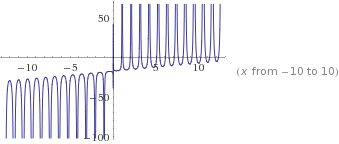
\includegraphics{lab3_1.png}
	\caption{$f(x)$}
	\label{lab3_1}
\end{figure}

\begin{figure}[h]
	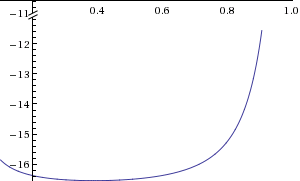
\includegraphics{lab3_2.png}
	\caption{$f(x), x=[0.1, 1]$}
	\label{lab3_2}
\end{figure}

\section{Метод бисекции}

\begin{table}[!h]
\begin{tabular}{l|l|l}
	$\varepsilon$  	& i 	& x \\
	\hline
	0.0001 			& 14& 0.966876220703125\\
	0.0000001		& 24& 0.9669269144535065\\
	0.0000000001	& 34& 0.9669269093719778\\
\end{tabular}
\end{table}

\section{Метод Ньютона}
\begin{table}[!h]
\begin{tabular}{l|l|l}
	$\varepsilon$  	& i & x \\
	\hline
	0.0001 			& 8	& 13.252873093705627\\
	0.0000001		& 9	& 13.25287309188221\\
	0.0000000001	& 10& 13.252873091882208\\
\end{tabular}
\end{table}

Метод Ньютона, при начальном $x_{0} = 0.55$ не сходится (см. Рис.\ref{lab3_3}).
\begin{figure}[!h]
	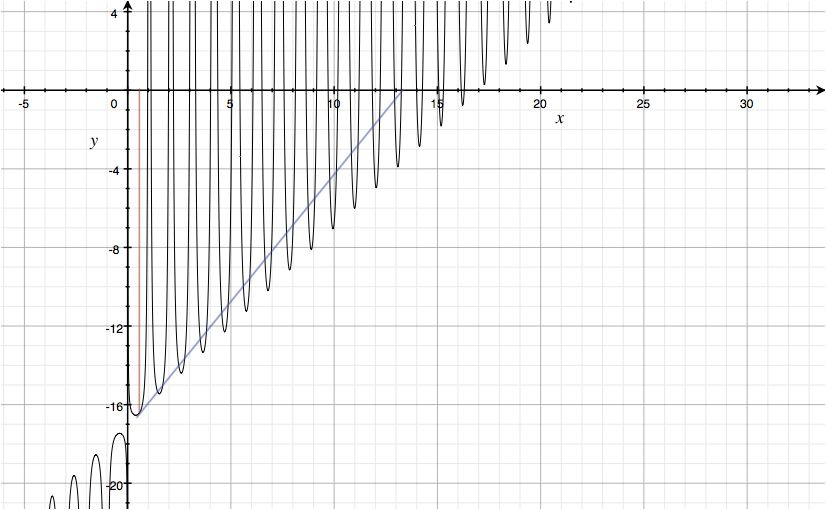
\includegraphics[width=11cm]{lab3_3.png}
	\caption{Первые шаги поиска корня методом Ньютона для функции}
	\label{lab3_3}
\end{figure}


\begin{table}[!h]
\begin{tabular}{l|l|l}
	$\varepsilon$  	& i 	& x \\
	\hline
	0.0001 			& 13& 0.9669269098589153\\
	0.0000001		& 14& 0.9669269093418339\\
	0.0000000001	& 15& 0.9669269093418338\\
\end{tabular}
\caption{Ньютон для заданного интервала $x = [0.1, 1]$}
\label{adj_neuton}
\end{table}

\section{Вывод}
По сравнению с методом Ньютона, метод бисекции имеет очень большой прирост
итераций, при увеличении точности.
Однако, в данной лабораторной работе хорошо продемонстрирован недостаток метода
Ньютона: результат сильно зависит от исходной точки.
Корень найден, но он находится не в запрашиваемом интервале.
Предугадать, к какому корню приведет начальное приближение можно вычислив
бассейны Ньютона, или проанализировав функцию.
Мы использовали начальное приближение $x_{0} = 0.91$ для того чтобы попасть в
требуемый условием задачи интервал (См. Табл.\ref{adj_neuton})- но такое
приближение, было выведено не алгоритмтчески, что усложнило использование данного метода.

\section{Исходный код}
\subsection{Метод бисекции}
\begin{lstlisting}
var a = 0.1;
var b = 1;
//var e = 0.0001
//var e = 0.0000001
var e = 0.0000000001
console.log(bisection(a, b, e))

function f(x) {
	return x / (Math.pow(Math.sin(3*x), 2)) - 17// my homework
}

function bisection(a, b, e) {
	var i = 1
	do {
		var x = (a+b)/2
		console.log('it: ' + i)
		console.log('x: ' + x + ', ab = [' + a + ', ' + b + ']')
		if(f(a) * f(x) <= 0) {
			b = x
		} else {
			a = x
		}
		i++
	} while (Math.abs(b - a) > e)
	return x
}
\end{lstlisting}


\subsection{Метод Ньютона}
\begin{lstlisting}
function neuton(a, b, e) {
	var i = 0;
	var x = (a+b)/2
//	var x = 0.91
	var xNew
	console.log('x: ' + x )
	do {
		xNew = ( x - (f(x) / fD(x)));
		i++;
		var delta = Math.abs(x - xNew)

		console.log('it: ' + i)
		console.log('xNew: ' + xNew +'  delta: ' + delta)
		x = xNew
	} while(delta > e);
	return x;
}

function f(x) {
	return x / (Math.pow(Math.sin(3*x), 2)) - 17 // my homework
}

function fD(x) {
	return (1 - 6*x/ Math.tan(3*x)) * (1/Math.pow(Math.sin(3*x), 2)) // my homework
}
var a = 0.1;
var b = 1;
var e = 0.0001
//var e = 0.0000001
//var e = 0.0000000001
neuton(a, b, e);

\end{lstlisting}
\end{document}